\documentclass{article}
\usepackage{bm}
\usepackage{amsmath}

\title{Two-Dimensional Dendritic Growth Using Phase-Field Model \\ Design Document}
\date{2015-Nov-24}
\author{CS 294-73 Group H}

\begin{document}
\pagenumbering{arabic}
\maketitle
    
\section{Discretization Methods and Numerical Schemes}
Recall the governing equations:
\begin{equation}
\begin{cases}
\frac{\partial u}{\partial t} =&D\nabla^2u+\frac{1}{2}\frac{\partial\phi}{\partial t} \\
\tau\frac{\partial \phi}{\partial t} =&\nabla(W^2\nabla\phi)+\partial_x[|\nabla\phi|^2W\partial_{\phi_x}W]+\partial_y[|\nabla\phi|^2W\partial_{\phi_y}W] \\
&+\phi(1-\phi^2)-\lambda u(1-\phi^2)^2 \\
W=&\eta((1-3\epsilon)+4\epsilon\frac{\phi_x^4+\phi_y^4}{|\nabla\phi|^4})
\end{cases}
\end{equation}

A 2nd order central difference scheme will be used for spatial discretization while a 4th order Runge-Kutta scheme for time integration. 

The final computational solution consists of time dependent phase field ($\phi$) and dimensionless temperature field ($u$) in the form of vtk files.

\section{Algorithm and Flow Chart}
\begin{figure}[h]
\begin{center}
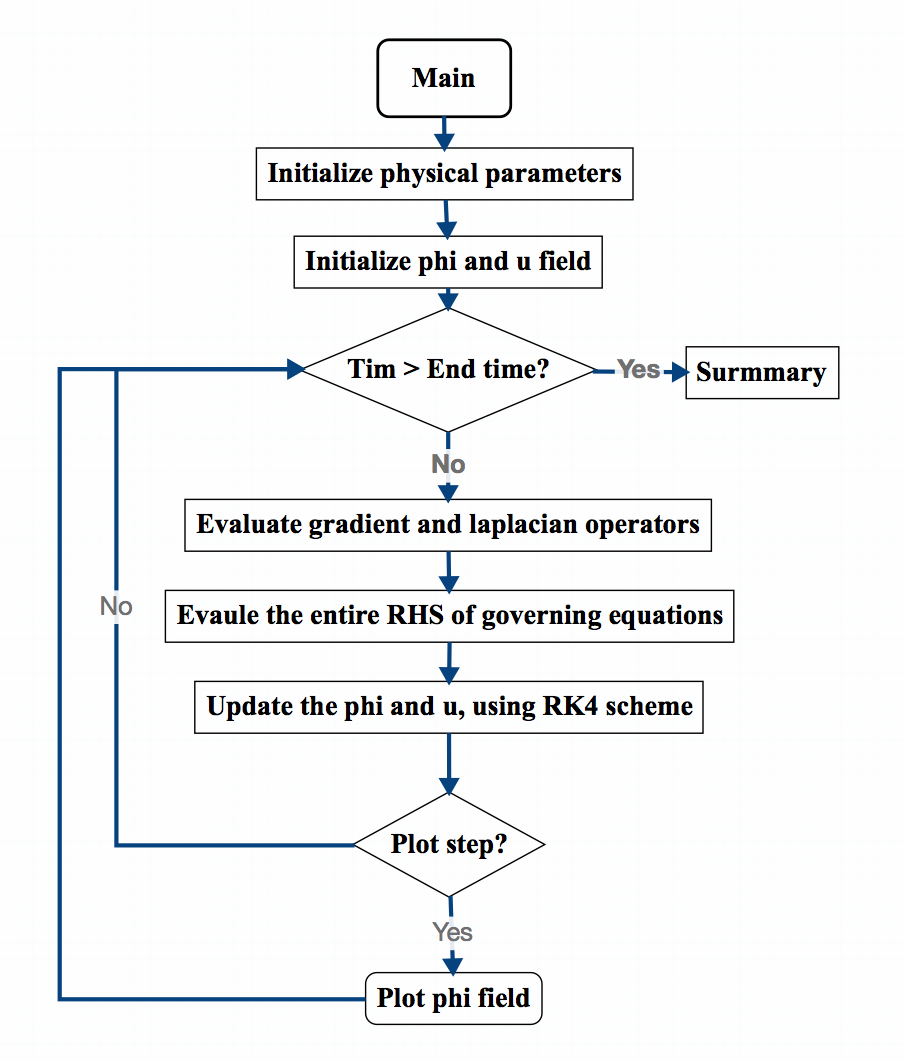
\includegraphics[width=0.65\textwidth]{flowchart_v_1} % Include the image placeholder.png
\caption{Figure caption.}
\end{center}
\end{figure}
        \par \ 
        \par 1. Initialize the modeling parameter including: timestep dt,time t, grid dh, domain size L, etc.  Initialize the $\phi$ and $u$ field.
        \par 2. During one step, we calculate the gradient and laplacian by 
        \par 3. Calculate the orientation angle $\theta$, and then the $W$
        \par 4. make RHS of $\phi$ euqation, update $\phi$ and then update $u$ by RK4
        \par 5. Plot intermidiate time step contour of  $\phi$ and $u$
  
\section{Software Design}
The following existing classes will be directly utilized:
\begin{description}
\item[Point]
\item[Box]
\item[RectMDarray]
\item[RK4]
\item[VisitWriter]
\item[]
\end{description}

\subsection{Analysis}
\begin{description}
\item[Output]
\item[Timer]
\end{description} 
	
\section{Optimization}
\section{Parameter Study} 
\section{Work Contribution} 

\end{document}